\documentclass{article}

%\usepackage[T1]{fontenc}
%\usepackage[utf8]{inputenc}
%\usepackage{polski}
\usepackage[utf8]{inputenc}
\usepackage{polski}
\usepackage[polish]{babel}
\usepackage{mathtools}
\usepackage[thinc]{esdiff}
\usepackage{graphicx} 

\usepackage{float}

\usepackage{geometry}

\begin{document}
\newgeometry{tmargin =3cm, bmargin=3cm, lmargin=3cm, rmargin=3cm}
\begin{tabular}{|c|c|c|}
\hline 
\multicolumn{3}{|c|}{\huge Sprawozdanie } \\ 
\hline 
\multicolumn{3}{|c|}{\LARGE Projekt 2 NMTS - Odwrócone wahadło} \\ 
\hline 
\Large Przygotowali: &\Large Piotr Pietruszka 171842 &\Large Marcin Wankiewicz 172118  \\ 
\hline 
\Large Kierunek: ACiR  \\ 
\hline 
 
\end{tabular} 

\section{Zlinearyzowany model stanowy}

Równania różniczkowe opisujące dynamikę układu przedstawiono w: \ref{eq:dyn}.
\begin{equation}\label{eq:dyn}
 \begin{array}{l}
  (M+m) \ddot{y} + b\dot{y} = F + mL\theta^2 \sin\theta - mL\ddot{\theta}\cos\theta \\
  (I + mL^2)\ddot{\theta} = mgL\sin\theta - mL\ddot{y}\cos\theta
 \end{array}
\end{equation}
W celu linearyzacji wokół punktu $\theta=0$, dla równań \ref{eq:dyn} użyto następujące przybliżenia: \ref{eq:appr}.
\begin{equation}\label{eq:appr}
 \begin{array}{l}
  \cos\theta = 1,\;  \sin\theta=\theta, \; \dot{\theta}^2 = 0
 \end{array}
\end{equation}

W wyniku otrzymano model stanowy (macierze zgodnie ze standardowymi oznaczeniami): \ref{eq:ss}, gdzie wektor stanu $\textbf{x}$ jest zdefiniowany w \ref{eq:sv}, a wejściem jest siła $F$ działająca na wózek.

\begin{equation}\label{eq:ss}
 \begin{array}{l}
  \mathbf{A} = \begin{bmatrix}  0 & 1 & 0 & 0 \\
  							   0 & -\frac{(I+mL^2)b}{I(M+m) + MmL^2} & -\frac{m^2gL^2}{I(M+m) + MmL^2} & 0 \\
  							   0 & 0 & 0 & 1 \\
  							   0 & \frac{bmL}{I(M+m) + MmL^2} & \frac{gmL(M+m)}{I(M+m) + MmL^2} & 0 \\ 
  			   \end{bmatrix} \\ \\
  			   
  \mathbf{B} = \begin{bmatrix} 0 \\ \frac{I + mL^2}{I(M+m) + MmL^2} \\ 0 \\ -\frac{mL}{I(M+m) + MmL^2} \end{bmatrix} \\ \\
  
  \mathbf{C} = \begin{bmatrix}  1 & 0 & 0 & 0 \\
  							   0 & 1 & 0 & 0 \\
  							   0 & 0 & 1 & 0 \\
  							   0 & 0 & 0 & 1 \\ 
  			   \end{bmatrix} \\ \\
  
  \mathbf{D} = \begin{bmatrix} 0 \end{bmatrix} \\
\end{array}
\end{equation}

\begin{equation}\label{eq:sv}
 \begin{array}{l}
	\mathbf{x} = 
	\begin{bmatrix} 
	  y \\ \dot{y} \\ \theta \\ \dot{\theta} 
	\end{bmatrix} 
 \end{array}
\end{equation}
Po podstawieniu wartości liczbowych: \ref{eq:ss_val}.

\begin{equation}\label{eq:ss_val}
 \begin{array}{l}
  \mathbf{A} = \begin{bmatrix}  0 & 1 & 0 & 0 \\
  							   0 & -1.16896918\cdot10^{-2} & -2.81381031\cdot10^{-1} & 0 \\
  							  0 & 0 & 0 & 1 \\
  							   0 & 3.18809777\cdot10^{-2} & 2.75128119\cdot10^{1} & 0 \\ 
  			   \end{bmatrix} \\ \\
  			   
  \mathbf{B} = \begin{bmatrix} 0 \\ 0.11689692 \\ 0 \\ -0.31880978 \end{bmatrix} \\ \\
  
  \mathbf{C} = \begin{bmatrix} 1 & 0 & 0 & 0 \\
  							   0 & 1 & 0 & 0 \\
  							   0 & 0 & 1 & 0 \\
  							   0 & 0 & 0 & 1 \\ 
  			   \end{bmatrix} \\ \\
  
  \mathbf{D} = \begin{bmatrix} 0 \end{bmatrix} \\
\end{array}
\end{equation}

Celem sterowania jest osiągnięcie przez układ wartości: \ref{eq:goal}.
\begin{equation}\label{eq:goal}
 \begin{array}{l}
y_{des} = 2m \\
v_{des} = 0 m/s \\
\theta_{des} = 0 rad \\
\omega_{des} = 0 rad/s
\end{array}
\end{equation}

\section{Sprzężenie od stanu}

Aby zaimplementować sterownik sprzężenia od stanu, obliczona została macierz sterowalności $P_c$:
\begin{equation}\label{eq:pc_matrix}
\mathbf{P_c} = \begin{bmatrix}  0 & 1.16896918\cdot10^{-1} & -1.36648895\cdot10^{-3} & 8.97229975\cdot10^{-2} \\
  							   1.16896918\cdot10^{-1} & -1.36648895\cdot10^{-2} & 8.97229975\cdot10^{-3} & -2.09748165\cdot10^{-3} \\
  							  0 & -3.18809777\cdot10^{-1} & 3.72678804\cdot10^{-3} & -8.77139699 \\
  							   -3.18809777\cdot10^{-1} & 3.72678804\cdot10^{-3} & -8.77139699 & 1.05394875\cdot10^{-1} \\ 
  			   \end{bmatrix} \\ \\
\end{equation}

Pożądany wielomian charakterystyczny został arbitralnie ustalony na czterokrotny biegun w -1+0j:
\begin{equation}\label{eq:des_ch_poly}
 (s + 1)^4 = s^4 + 4s^3 + 6s^2 + 4s + 1
\end{equation}

Zgodnie z tym ustaleniem, policzona została macierz wzmocnień sterownika od stanu:
\begin{equation}\label{eq:k_matrix}
\mathbf{K} = \begin{bmatrix}  -0.31985099 & -1.37940394 & -105.23579869 & -13.01578145 \\
  			   \end{bmatrix} \\ \\
\end{equation}

Model stanowy układu ze sterownikiem ze sprzężeniem od stanu:
\begin{equation}\label{eq:_statefeedback_ss}
 \begin{array}{l}
  \mathbf{A} = \begin{bmatrix}  -3.98831031 & -2.98831031 & -3.98831031 & -3.98831031 \\
  							   -3.98831031 & -4 & -4.26969134 & -3.98831031 \\
  							   -3.98831031 & -3.98831031 & -3.98831031 & -2.98831031 \\
  							   -3.98831031 & -3.95642933 & 23.52450159 & -3.98831031 \\ 
  			   \end{bmatrix} \\ \\
  			   
  \mathbf{B} = \begin{bmatrix} 0 \\ 0.11689692 \\ 0 \\ -0.31880978 \end{bmatrix} \\ \\
  
  \mathbf{C} = \begin{bmatrix}  1 & 0 & 0 & 0 \\
  							   0 & 1 & 0 & 0 \\
  							   0 & 0 & 1 & 0 \\
  							   0 & 0 & 0 & 1 \\ 
  			   \end{bmatrix} \\ \\
  
  \mathbf{D} = \begin{bmatrix} 0 \end{bmatrix} \\
\end{array}
\end{equation}

Wyjścia układu ze sprzężeniem od stanu:
\begin{figure}[H]
    \centering
    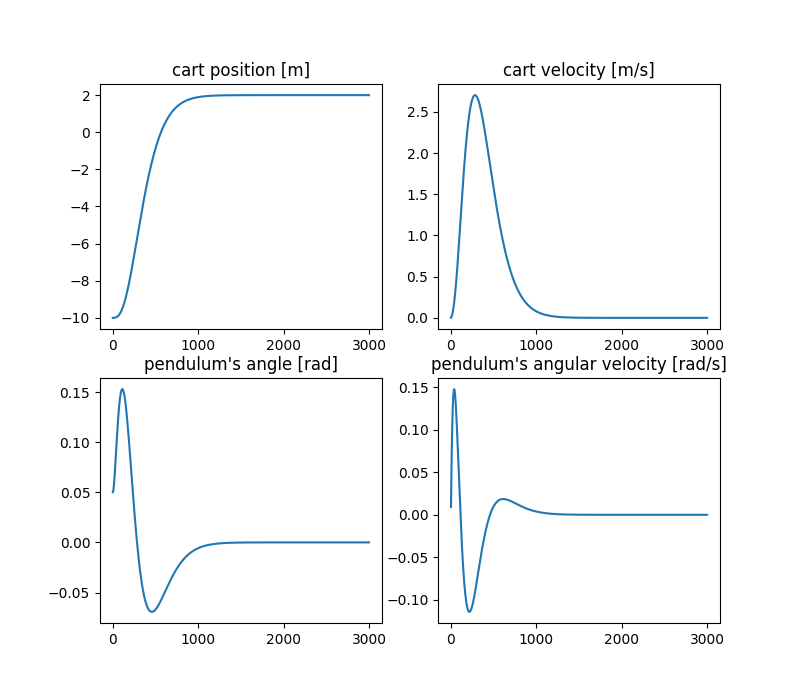
\includegraphics[width=0.7\textwidth]{img/statespace.png}
    \caption{Odpowiedzi układu ze sprzężeniem od stanu. Krok symulacji $dt=0.01$ s}
    \label{fig:state_space}
\end{figure}

Jak widać na wykresach, układ jest stabilny i osiąga wyznaczone w założeniach wartości (\ref{eq:goal}), po czym stabilnie je utrzymuje, co oznacza, że sterownik został dobrze zaprojektowany i spełnia swoją funkcję.

\section{LQR}

W tym rozdziale zostanie przedstawione kilka przypadków sterownika LQR, zgodnie z instrukcją projektu. Wszystkie wykresy zostaną narysowane w tej samej skali osi czasu, by łatwiej było porównać prędkości ustalania układów.

\subsection{Tanie sterowanie, droga precyzja}
W tym podrozdziale zakładamy, że sterowanie jest tanie w stosunku do precyzji sterowania. Na diagonali macierzy Q ustawione zostały na duże wartości:
\begin{equation}\label{eq:q1}
\mathbf{Q} = \begin{bmatrix}  1000 & 0 & 0 & 0 \\
  							  0 & 1000 & 0 & 0 \\
  							  0 & 0 & 1000 & 0 \\
  							  0 & 0 & 0 & 1000 \\ 
  			   \end{bmatrix} \\ \\
\end{equation}

Macierz R (w naszym przypadku jednostkowa) została ustawiona na relatywnie małą wartość:
\begin{equation}\label{eq:r1}
\mathbf{R} = \begin{bmatrix}  0.01
  			   \end{bmatrix} \\ \\
\end{equation}

Wartości własne macierzy A układu z takim sterownikiem wynoszą kolejno $-4.46851143\cdot10^{2}$, -8.90090168, $-4.21015551\cdot10^{-1}$ i 1.90614933.

Wyjścia układu:
\begin{figure}[H]
    \centering
    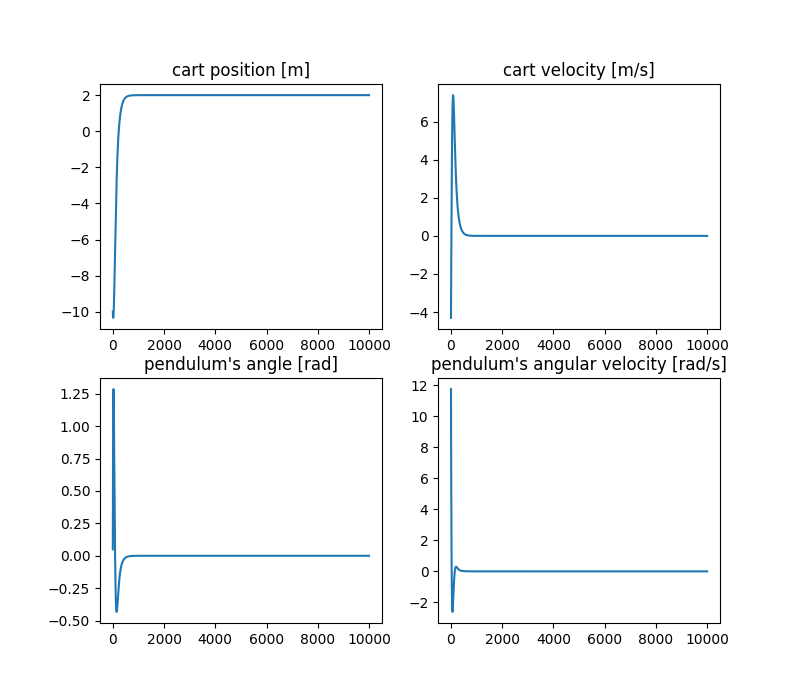
\includegraphics[width=0.7\textwidth]{img/drugi.png}
    \caption{Odpowiedzi ze sterownikiem LQR dla taniego sterowania. Krok symulacji $dt=0.01$ s}
    \label{fig:state_space}
\end{figure}

Jak widać na wykresie, przy sterowaniu duża waga przyłożona jest do dokładności stanu. Oznacza to, że stan jest szybko sprowadzany do wartości pożądanej. Dzieje się to jednak w sposób gwałtowny, co jest spowodowane użyciem dużych wartości siły pchającej wózek (duże wartości sterowania nie są w tym przypadku drogie). Oznacza to osiągnięcie dużych wartości np. przez prędkość wózka.

\subsection{Drogie sterowanie, tania precyzja}
W tym podrozdziale zakładamy, że sterowanie jest drogie w stosunku do precyzji sterowania. Tym razem na diagonali Q ustawione zostały mniejsze wartości:
\begin{equation}\label{eq:q1}
\mathbf{Q} = \begin{bmatrix}  1 & 0 & 0 & 0 \\
  							  0 & 0.1 & 0 & 0 \\
  							  0 & 0 & 0.1 & 0 \\
  							  0 & 0 & 0 & 0.1 \\ 
  			   \end{bmatrix} \\ \\
\end{equation}
Macierz R przeciwnie, została ustawiona na relatywnie dużą wartość:
\begin{equation}\label{eq:r1}
\mathbf{R} = \begin{bmatrix}  100
  			   \end{bmatrix} \\ \\
\end{equation}

Wartości własne macierzy A układu z takim sterownikiem wynoszą kolejno -33.45451986, -10.53878129, -0.4263347 oraz 1.9832387.

Wyjścia układu:
\begin{figure}[H]
    \centering
    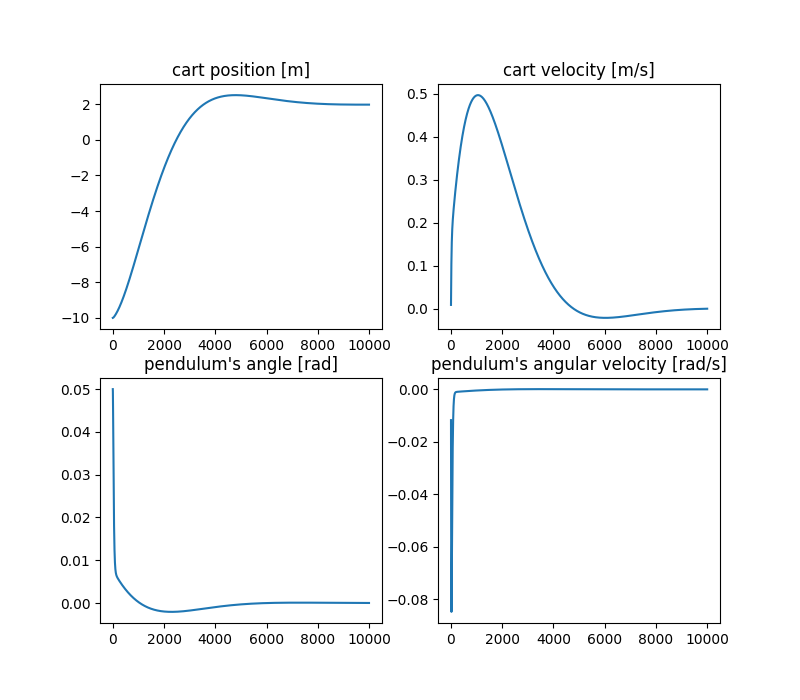
\includegraphics[width=0.7\textwidth]{img/pierwszy.png}
    \caption{Odpowiedzi ze sterownikiem LQR dla drogiego sterowania. Krok symulacji $dt=0.01$ s}
    \label{fig:state_space}
\end{figure}

W tym przypadku widać, że sterownik powoli steruje układem - czyli zadaje mu małe wartości siły pchającej wózek, gdyż sterowanie jest drogie.

\subsection{Droga prędkość wózka}
W tym podrozdziale zakładamy, że jedynie prędkość wózka jest droga w stosunku do precyzji sterowania. W macierzy Q tylko jedna wartość jest znacznie większa od pozostałych - ta odpowiedzialna za drugą zmienną stanu, prędkość wózka.
\begin{equation}\label{eq:q1}
\mathbf{Q} = \begin{bmatrix}  1 & 0 & 0 & 0 \\
  							  0 & 1000 & 0 & 0 \\
  							  0 & 0 & 0.1 & 0 \\
  							  0 & 0 & 0 & 0.1 \\ 
  			   \end{bmatrix} \\ \\
\end{equation}

Pierwszą wartość (odpowiedzialną za pozycję wózka) można jeszcze bardziej zmniejszyć, ale powoduje to znaczne rozciągnięcie wykresu w czasie - jest to naszym zdaniem dobry kompromis. Macierz R podobnie jak w poprzednim przypadku, została ustawiona na relatywnie małą wartość:
\begin{equation}\label{eq:r1}
\mathbf{R} = \begin{bmatrix}  0.1
  			   \end{bmatrix} \\ \\
\end{equation}

Wartości własne macierzy A układu z takim sterownikiem wynoszą kolejno -80.52898755, -9.40154754, -0.42325244 oraz 1.93852224.

Wyjścia układu:
\begin{figure}[H]
    \centering
    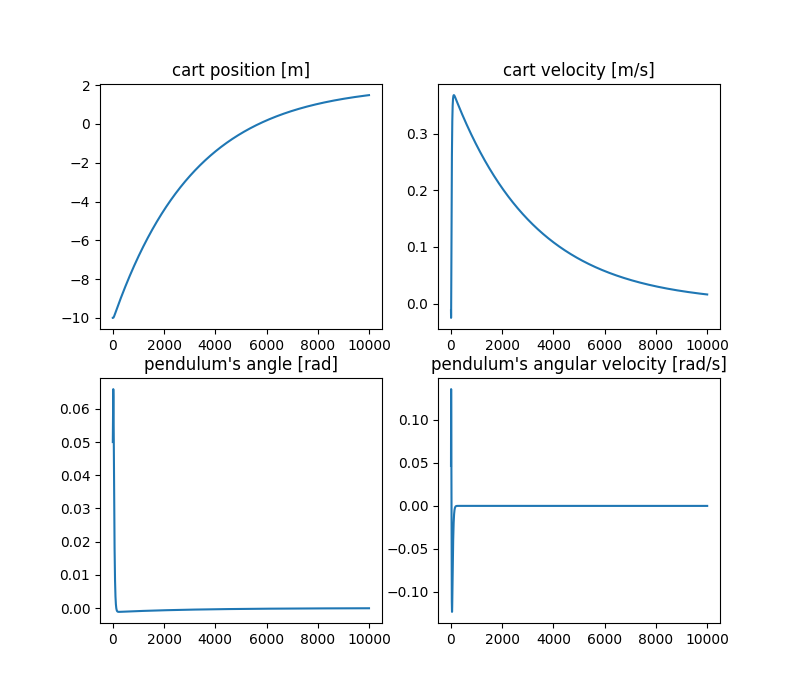
\includegraphics[width=0.7\textwidth]{img/trzeci.png}
    \caption{Odpowiedzi ze sterownikiem LQR dla drogiej prędkości wózka. Krok symulacji $dt=0.01$ s}
    \label{fig:state_space}
\end{figure}

W tym przypadku dążymy jedynie do zminimalizowania wartości sygnału prędkości wózka. Jej maksymalna wartość w tym przypadku to nieco ponad 0.3, a w pozostałych odpowiednio około 7 i 0.5. Pozostałe sygnały nie są tak restrykcyjnie ograniczane, na przykład kąt wychylenia wahadła oraz jego prędkość kątowa - są nieznacznie większe niż w drugim przypadku. Jest to swojego rodzaju kompromis pomiędzy szybkim ustaleniem prędkości do stanu ustalonego, a jej maksymalną wartością. Założenie projektowe zostało spełnione, ograniczyliśmy jedynie prędkość wózka, ponieważ jest droga.

\section{Wnioski z realizacji projektu}
Sterownik ze sprzężeniem od stanu poradził sobie bardzo dobrze z wysterowaniem układu, jednak bardzo trudno jest projektować go dla założeń typu "prędkość wózka jest droga, trzeba ją ograniczyć". Do tego celu idealnie nadaje się sterownik LQR. Jeśli precyzja sterowania dla danej zmiennej stanu jest dla nas istotna, to należy w macierzy Q ustawić odpowiednio większą wartość na miejscu w diagonali odpowiadającej tej zmiennej. Jeżeli natomiast sterowanie jest dla nas drogie, zwiększamy wartości w macierzy R (w naszym przypadku był to skalar, więc po prostu wartość R). Zaprezentowane przypadki dobrze pokazują działanie i znaczenie poszczególnych parametrów przy projektowaniu sterownika LQR i prezentują wadę sterowania ze sprzężeniem od stanu w stosunku do LQR.

\end{document}